
\documentclass[aspectratio=169,10pt]{beamer}

% Modern, sleek theme setup
\usetheme{metropolis}
\usecolortheme{owl}
\definecolor{solanagreen}{RGB}{20, 241, 149}
\definecolor{solanapurple}{RGB}{153, 69, 255}
\definecolor{darkblue}{RGB}{25, 35, 66}
\definecolor{neonblue}{RGB}{77, 171, 247}

% Packages
\usepackage{graphicx}
\usepackage{hyperref}
\usepackage{listings}
\usepackage{amsmath}
\usepackage{fontawesome5}
\usepackage{tikz}
\usepackage{tcolorbox}
\usepackage{anyfontsize}
\usepackage{xcolor}
\usepackage{varwidth}

\usetikzlibrary{arrows.meta,shapes,positioning,shadows,trees,decorations.pathmorphing,backgrounds,fit,patterns,calc}

% Custom styling
\setbeamercolor{background canvas}{bg=darkblue}
\setbeamercolor{frametitle}{fg=white}
\setbeamercolor{title}{fg=solanagreen}
\setbeamercolor{subtitle}{fg=white}
\setbeamercolor{normal text}{fg=white}
\setbeamercolor{itemize item}{fg=solanagreen}
\setbeamercolor{itemize subitem}{fg=neonblue}
\setbeamercolor{section in toc}{fg=solanagreen}

% Ensure content fits within the page
\setbeamersize{text margin left=10pt,text margin right=10pt}

% Title info
\title{\textbf{\LARGE{SHADOW BOOK}}}
\subtitle{\Large{An orderbook where even the matching engine can't see your trades}}
\author{\textbf{Kyle Koshiyama} \& \textbf{Mads Christensen}}
\date{Solana Hackathon 2025}
\logo{\includegraphics[width=1cm]{solana-logo}}

\begin{document}

% Title slide with futuristic animation effect
\begin{frame}[plain]
\begin{tikzpicture}[remember picture, overlay, scale=0.95]
    % Background gradient
    \fill[left color=darkblue, right color=black] (current page.south west) rectangle (current page.north east);
    
    % Animated network pattern (reduced number and scaled)
    \foreach \i in {1,...,15} {
        \pgfmathsetmacro{\x}{random(0,90)/10}
        \pgfmathsetmacro{\y}{random(0,60)/10}
        \pgfmathsetmacro{\r}{random(10,20)/100}
        \node[circle, fill=solanagreen, opacity=0.2, minimum size=\r cm] at (\x,\y) {};
    }
    
    % Connected lines (reduced)
    \foreach \i in {1,...,10} {
        \pgfmathsetmacro{\x}{random(0,90)/10}
        \pgfmathsetmacro{\y}{random(0,60)/10}
        \pgfmathsetmacro{\xx}{random(0,90)/10}
        \pgfmathsetmacro{\yy}{random(0,60)/10}
        \draw[solanapurple, opacity=0.1] (\x,\y) -- (\xx,\yy);
    }
    
    % Lock icon in the background (scaled down)
    \node[opacity=0.1, scale=7] at (5,0) {\faLock};
\end{tikzpicture}

\vspace{1cm}
\begin{center}
    \begin{tcolorbox}[colback=darkblue, colframe=solanagreen, width=0.8\textwidth, arc=5mm, boxrule=1.5pt]
        \vspace{0.3cm}
        \centering
        {\fontsize{36}{40}\selectfont\textcolor{solanagreen}{\textbf{SHADOW}}\textcolor{white}{\textbf{BOOK}}}\\[0.3cm]
        {\Large\textcolor{white}{Trade in the dark. Execute in the light.}}\\[0.2cm]
        \textcolor{neonblue}{\faLock \quad \faExchange \quad \faShieldAlt \quad \faLock}
        \vspace{0.3cm}
    \end{tcolorbox}
    \vspace{0.3cm}
    {\large\textcolor{white}{Kyle Koshiyama \& Mads Christensen}}\\[0.2cm]
    {\textcolor{solanagreen}{Solana Hackathon 2025}}
\end{center}
\end{frame}

% Stylish Table of Contents
\begin{frame}[plain]
\begin{tikzpicture}[remember picture, overlay, scale=0.95]
    % Background gradient
    \fill[left color=darkblue, right color=black!90] (current page.south west) rectangle (current page.north east);
    
    % Circuit board pattern (reduced)
    \draw[solanapurple, opacity=0.05, line width=0.5pt] (-1,-1) grid[step=0.7] (12,8);
    \foreach \i in {1,...,8} {
        \pgfmathsetmacro{\x}{random(0,90)/10}
        \pgfmathsetmacro{\y}{random(0,60)/10}
        \node[circle, draw=solanagreen, opacity=0.1, minimum size=0.2cm] at (\x,\y) {};
    }
\end{tikzpicture}

\vspace{0.3cm}
\begin{center}
    \begin{tcolorbox}[colback=darkblue, colframe=solanagreen, width=0.8\textwidth, arc=5mm, boxrule=1.5pt]
        \centering
        {\fontsize{26}{28}\selectfont\textcolor{solanagreen}{\faMapSigns} \textcolor{white}{\textbf{MISSION BRIEFING}}}
    \end{tcolorbox}
\end{center}
\begin{columns}[T,onlytextwidth]
    \column{0.48\textwidth}
    \begin{tcolorbox}[colback=darkblue!80, colframe=neonblue, width=\textwidth, arc=3mm, boxsep=0.1cm]
        \textcolor{solanagreen}{\faExclamationTriangle} \textcolor{white}{\textbf{THE PROBLEM}}\\[0.05cm]
        \textcolor{white}{Exposed trading data = vulnerable markets}
    \end{tcolorbox}
    \vspace{0.1cm}
    \begin{tcolorbox}[colback=darkblue!80, colframe=neonblue, width=\textwidth, arc=3mm, boxsep=0.1cm]
        \textcolor{solanagreen}{\faLightbulb} \textcolor{white}{\textbf{THE SOLUTION}}\\[0.05cm]
        \textcolor{white}{FHE-powered invisible orderbook}
    \end{tcolorbox}
    \vspace{0.1cm}
    \begin{tcolorbox}[colback=darkblue!80, colframe=neonblue, width=\textwidth, arc=3mm, boxsep=0.1cm]
        \textcolor{solanagreen}{\faChartLine} \textcolor{white}{\textbf{MARKET OPPORTUNITY}}\\[0.05cm]
        \textcolor{white}{\$50B+ DeFi market craving privacy}
    \end{tcolorbox}
    
    \column{0.48\textwidth}
    \begin{tcolorbox}[colback=darkblue!80, colframe=neonblue, width=\textwidth, arc=3mm, boxsep=0.1cm]
        \textcolor{solanagreen}{\faLaptop} \textcolor{white}{\textbf{LIVE DEMO}}\\[0.05cm]
        \textcolor{white}{See the invisible in action}
    \end{tcolorbox}
    \vspace{0.1cm}
    \begin{tcolorbox}[colback=darkblue!80, colframe=neonblue, width=\textwidth, arc=3mm, boxsep=0.1cm]
        \textcolor{solanagreen}{\faDollarSign} \textcolor{white}{\textbf{BUSINESS MODEL}}\\[0.05cm]
        \textcolor{white}{How we capture value}
    \end{tcolorbox}
    \vspace{0.1cm}
    \begin{tcolorbox}[colback=darkblue!80, colframe=neonblue, width=\textwidth, arc=3mm, boxsep=0.1cm]
        \textcolor{solanagreen}{\faUsers} \textcolor{white}{\textbf{TEAM}}\\[0.05cm]
        \textcolor{white}{FHE + Solana experts ready to build}
    \end{tcolorbox}
    \vspace{0.1cm}
    \begin{tcolorbox}[colback=darkblue!80, colframe=neonblue, width=\textwidth, arc=3mm, boxsep=0.1cm]
        \textcolor{solanagreen}{\faRoad} \textcolor{white}{\textbf{ROADMAP}}\\[0.05cm]
        \textcolor{white}{From hackathon to revolution}
    \end{tcolorbox}
\end{columns}
\end{frame}

% Problem
\begin{frame}[plain]
\begin{tikzpicture}[remember picture, overlay, scale=0.95]
    % Background with hacker aesthetic
    \fill[left color=darkblue, right color=black] (current page.south west) rectangle (current page.north east);
    
    % Matrix-style falling code effect (reduced)
    \foreach \i in {1,...,15} {
        \pgfmathsetmacro{\x}{random(0,90)/10}
        \pgfmathsetmacro{\y}{random(-10,60)/10}
        \pgfmathsetmacro{\op}{random(10,20)/100}
        \node[text=solanagreen, opacity=\op] at (\x,\y) {\tiny{01}};
    }
    
    % Hacker silhouette (scaled down)
    \node[anchor=south east, opacity=0.1, scale=0.7] at (current page.south east) {
        \faUser
    };
\end{tikzpicture}

\vspace{0.2cm}
\begin{center}
    \begin{tcolorbox}[colback=darkblue, colframe=solanapurple, width=0.8\textwidth, arc=5mm, boxrule=1.5pt]
        {\fontsize{26}{28}\selectfont\textcolor{white}{\textbf{THE}} \textcolor{solanagreen}{\textbf{PROBLEM}}}
    \end{tcolorbox}
\end{center}

\vspace{0.3cm}
\begin{columns}[T,onlytextwidth]
    \column{0.55\textwidth}
    \begin{tcolorbox}[colback=darkblue!80, colframe=solanagreen, width=\textwidth, arc=3mm, title=\textcolor{white}{\textbf{TRANSPARENT ORDERBOOKS = VULNERABLE}}]
        \begin{itemize}
            \item[\textcolor{solanagreen}{\faEye}] \textcolor{white}{\textbf{Everyone sees your trades}}
            \item[\textcolor{solanagreen}{\faRunning}] \textcolor{white}{\textbf{Front-running attacks}}
            \item[\textcolor{solanagreen}{\faBinoculars}] \textcolor{white}{\textbf{Whale tracking}}
            \item[\textcolor{solanagreen}{\faChartLine}] \textcolor{white}{\textbf{Market manipulation}}
        \end{itemize}
    \end{tcolorbox}
    
    \column{0.4\textwidth}
    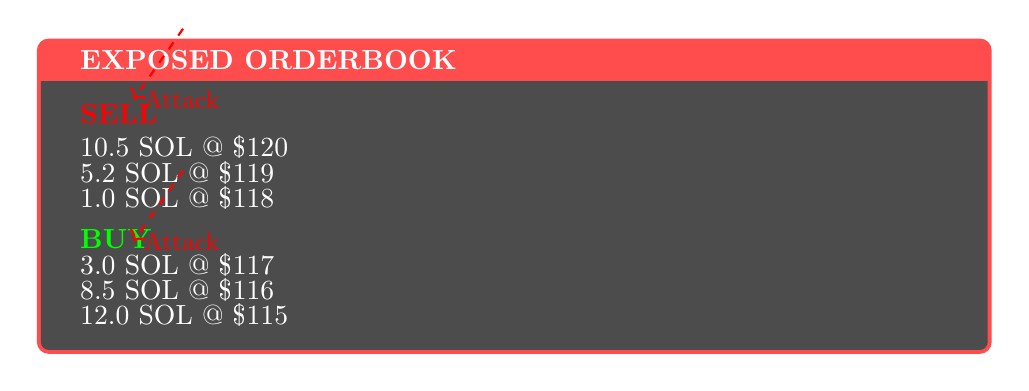
\begin{tikzpicture}[scale=0.9]
        % Orderbook visualization with exposed data
        \node[anchor=north west] at (0,0) {
            \begin{tcolorbox}[colback=black!70, colframe=red!70, width=\textwidth, title=\textcolor{white}{\textbf{EXPOSED ORDERBOOK}}]
                \textcolor{red}{\textbf{SELL}}\\
                \textcolor{white}{10.5 SOL @ \$120}\\[-0.1cm]
                \textcolor{white}{5.2 SOL @ \$119}\\[-0.1cm]
                \textcolor{white}{1.0 SOL @ \$118}\\[0.1cm]
                \textcolor{green}{\textbf{BUY}}\\[-0.1cm]
                \textcolor{white}{3.0 SOL @ \$117}\\[-0.1cm]
                \textcolor{white}{8.5 SOL @ \$116}\\[-0.1cm]
                \textcolor{white}{12.0 SOL @ \$115}
            \end{tcolorbox}
        };
        
        % Attack arrows (shortened)
        \draw[->, thick, red, dashed] (2.2,0) -- (1.5,-1) node[right, text=red, font=\small] {Attack};
        \draw[->, thick, red, dashed] (2.2,-2) -- (1.5,-3) node[right, text=red, font=\small] {Attack};
    \end{tikzpicture}
\end{columns}

\vspace{0.2cm}
\begin{center}
    \begin{tcolorbox}[colback=red!50, colframe=red!90, width=0.8\textwidth, arc=3mm]
        \centering
        \textcolor{white}{\textbf{"In DeFi, if your trade is visible, it's vulnerable"}}
    \end{tcolorbox}
\end{center}
\end{frame}

% Solution
\begin{frame}[plain]
\begin{tikzpicture}[remember picture, overlay, scale=0.95]
    % Background with futuristic tech aesthetic
    \fill[left color=darkblue, right color=black] (current page.south west) rectangle (current page.north east);
    
    % Digital circuit pattern (reduced)
    \foreach \i in {1,...,12} {
        \pgfmathsetmacro{\x}{random(0,90)/10}
        \pgfmathsetmacro{\y}{random(0,60)/10}
        \pgfmathsetmacro{\xx}{\x+random(5,10)/10}
        \pgfmathsetmacro{\yy}{\y+random(5,10)/10}
        \draw[solanagreen, opacity=0.05] (\x,\y) -- (\xx,\yy);
    }
    
    % Lock icon in the background (scaled down)
    \node[opacity=0.08, scale=10] at (9,1) {\faLock};
\end{tikzpicture}

\vspace{0.2cm}
\begin{center}
    \begin{tcolorbox}[colback=darkblue, colframe=solanagreen, width=0.8\textwidth, arc=5mm, boxrule=1.5pt]
        {\fontsize{26}{28}\selectfont\textcolor{white}{\textbf{THE}} \textcolor{solanagreen}{\textbf{SOLUTION}}}
    \end{tcolorbox}
\end{center}

\vspace{0.2cm}
\begin{columns}[T,onlytextwidth]
    \column{0.48\textwidth}
    \begin{tcolorbox}[colback=darkblue!80, colframe=solanagreen, width=\textwidth, arc=3mm, title=\textcolor{white}{\textbf{SHADOWBOOK TECHNOLOGY}}]
        \begin{itemize}
            \item[\textcolor{solanagreen}{\faLock}] \textcolor{white}{\textbf{Fully Homomorphic Encryption}}
            \item[\textcolor{solanagreen}{\faExchange}] \textcolor{white}{\textbf{Encrypted Matching Engine}}
            \item[\textcolor{solanagreen}{\faBolt}] \textcolor{white}{\textbf{Solana-Powered Settlement}}
            \item[\textcolor{solanagreen}{\faShieldAlt}] \textcolor{white}{\textbf{Zero-Knowledge Proofs}}
        \end{itemize}
    \end{tcolorbox}
    
    \column{0.48\textwidth}
    \begin{tikzpicture}[scale=0.9]
        % Encrypted orderbook visualization
        \node[anchor=north west] at (0,0) {
            \begin{tcolorbox}[colback=black!70, colframe=solanagreen!70, width=\textwidth, title=\textcolor{white}{\textbf{ENCRYPTED ORDERBOOK}}]
                \textcolor{red}{\textbf{SELL}}\\[-0.1cm]
                \textcolor{white}{********** @ ****}\\[-0.1cm]
                \textcolor{white}{********** @ ****}\\[-0.1cm]
                \textcolor{white}{********** @ ****}\\[0.1cm]
                \textcolor{green}{\textbf{BUY}}\\[-0.1cm]
                \textcolor{white}{********** @ ****}\\[-0.1cm]
                \textcolor{white}{********** @ ****}\\[-0.1cm]
                \textcolor{white}{********** @ ****}
            \end{tcolorbox}
        };
        
        % Shield icon (scaled down)
        \node[text=solanagreen, opacity=0.2, scale=2] at (2.2,-2) {\faShieldAlt};
    \end{tikzpicture}
\end{columns}

\vspace{0.2cm}
\begin{center}
    \begin{tcolorbox}[colback=solanagreen!40!darkblue!60, colframe=solanagreen, width=0.8\textwidth, arc=3mm]
        \centering
        \textcolor{white}{\textbf{"Trade without revealing your strategy - even to the matching engine"}}
    \end{tcolorbox}
\end{center}
\end{frame}

% How it works
\begin{frame}[plain]
\begin{tikzpicture}[remember picture, overlay, scale=0.95]
    % Background with tech circuit aesthetic
    \fill[left color=darkblue, right color=black] (current page.south west) rectangle (current page.north east);
    
    % Circuit board pattern (reduced)
    \draw[solanapurple, opacity=0.05, line width=0.5pt] (-1,-1) grid[step=1] (12,8);
\end{tikzpicture}

\vspace{0.2cm}
\begin{center}
    \begin{tcolorbox}[colback=darkblue, colframe=neonblue, width=0.8\textwidth, arc=5mm, boxrule=1.5pt]
        {\fontsize{26}{28}\selectfont\textcolor{white}{\textbf{HOW}} \textcolor{solanagreen}{\textbf{IT WORKS}}}
    \end{tcolorbox}
\end{center}

\vspace{0.3cm}
\begin{center}
\begin{tikzpicture}[node distance=1.2cm, auto, thick, scale=0.85, transform shape,
    block/.style={rectangle, draw=solanagreen, rounded corners, fill=darkblue!80, text width=2.8cm, align=center, minimum height=0.9cm},
    line/.style={draw, -latex', line width=1pt, solanagreen}]
    
    % Nodes (reduced size)
    \node[block] (client) {\textcolor{white}{\textbf{1. CLIENT}}\\\textcolor{neonblue}{Encrypt orders with FHE}};
    \node[block, right=1.8cm of client] (submit) {\textcolor{white}{\textbf{2. SUBMIT}}\\\textcolor{neonblue}{Send encrypted orders}};
    \node[block, below=0.8cm of submit] (match) {\textcolor{white}{\textbf{3. MATCH}}\\\textcolor{neonblue}{Homomorphic comparison}};
    \node[block, left=1.8cm of match] (execute) {\textcolor{white}{\textbf{4. EXECUTE}}\\\textcolor{neonblue}{Settlement on Solana}};
    \node[block, below=0.8cm of execute] (decrypt) {\textcolor{white}{\textbf{5. DECRYPT}}\\\textcolor{neonblue}{Only by order owner}};
    
    % Connections
    \path[line] (client) -- (submit);
    \path[line] (submit) -- (match);
    \path[line] (match) -- (execute);
    \path[line] (execute) -- (decrypt);
    \path[line] (decrypt) to[bend right=40] (client);
    
    % Icons
    \node[above=0.1cm of client, text=solanagreen] {\large\faLock};
    \node[above=0.1cm of submit, text=solanagreen] {\large\faPaperPlane};
    \node[above=0.1cm of match, text=solanagreen] {\large\faExchange};
    \node[above=0.1cm of execute, text=solanagreen] {\large\faBolt};
    \node[above=0.1cm of decrypt, text=solanagreen] {\large\faUnlock};
\end{tikzpicture}
\end{center}

\vspace{0.4cm}
\begin{tcolorbox}[colback=solanagreen!20, colframe=solanagreen, width=0.9\textwidth, arc=3mm, boxsep=0.2cm]
    \begin{varwidth}{\linewidth}
    \small\textbf{KEY INNOVATION:} \textcolor{white}{The matching engine operates directly on encrypted data using FHE, never seeing the actual prices or quantities. Only valid matches are executed, maintaining market integrity while preserving privacy.}
    \end{varwidth}
\end{tcolorbox}
\end{frame}

% Market opportunity
\begin{frame}[plain]
\begin{tikzpicture}[remember picture, overlay, scale=0.95]
    % Background with financial data aesthetic
    \fill[left color=darkblue, right color=black] (current page.south west) rectangle (current page.north east);
    
    % Market data pattern (reduced)
    \foreach \i in {1,...,20} {
        \pgfmathsetmacro{\x}{random(0,90)/10}
        \pgfmathsetmacro{\y}{random(0,60)/10}
        \pgfmathsetmacro{\op}{random(5,10)/100}
        \node[text=neonblue, opacity=\op] at (\x,\y) {\tiny{\$}};
    }
\end{tikzpicture}

\vspace{0.02cm}
\begin{center}
    \begin{tcolorbox}[colback=darkblue, colframe=neonblue, width=0.8\textwidth, arc=5mm, boxrule=1.5pt]
        {\fontsize{24}{26}\selectfont\textcolor{white}{\textbf{MARKET OPPORTUNITY}}}
    \end{tcolorbox}
\end{center}

\vspace{0.02cm}
\begin{columns}[T,onlytextwidth]
    \column{0.48\textwidth}
    \begin{tcolorbox}[colback=darkblue!80, colframe=neonblue, width=\textwidth, arc=3mm, title=\textcolor{white}{\textbf{DEFI MARKET SIZE}}]
        \begin{center}
            {\fontsize{20}{24}\selectfont\textcolor{solanagreen}{\$50B+}}\\[0.05cm]
            \textcolor{white}{Total Value Locked}\\[0.1cm]
            {\fontsize{20}{24}\selectfont\textcolor{solanagreen}{\$20B+}}\\[0.05cm]
            \textcolor{white}{Monthly DEX Volume}\\[0.1cm]
            {\fontsize{20}{24}\selectfont\textcolor{solanagreen}{78\%}}\\[0.05cm]
            \textcolor{white}{Users concerned about privacy}
        \end{center}
    \end{tcolorbox}
    
    \column{0.48\textwidth}
    \begin{tcolorbox}[colback=darkblue!80, colframe=neonblue, width=\textwidth, arc=3mm, title=\textcolor{white}{\textbf{TARGET SEGMENTS}}]
        \begin{itemize}
            \item[\textcolor{solanagreen}{\faBuilding}] \textcolor{white}{\textbf{Institutional traders}}\\[-0.2cm]
            \textcolor{white}{\small Seeking confidential execution}
            \item[\textcolor{solanagreen}{\faChartLine}] \textcolor{white}{\textbf{Crypto whales}}\\[-0.2cm]
            \textcolor{white}{\small Avoiding front-running}
            \item[\textcolor{solanagreen}{\faRobot}] \textcolor{white}{\textbf{Algorithmic strategies}}\\[-0.2cm]
            \textcolor{white}{\small Protecting proprietary signals}
            \item[\textcolor{solanagreen}{\faProjectDiagram}] \textcolor{white}{\textbf{DeFi protocols}}\\[-0.2cm]
            \textcolor{white}{\small Requiring private rebalancing}
        \end{itemize}
    \end{tcolorbox}
\end{columns}

\begin{center}
    \begin{tcolorbox}[colback=neonblue!50, colframe=neonblue, width=0.8\textwidth, arc=3mm, boxsep=0.1cm]
        \centering
        \textcolor{white}{\textbf{COMPETITIVE ADVANTAGE:} First-mover in FHE-based orderbooks on Solana}
    \end{tcolorbox}
\end{center}
\end{frame}

% Demo
\begin{frame}[plain]
\begin{tikzpicture}[remember picture, overlay, scale=0.95]
    % Background with tech aesthetic
    \fill[left color=darkblue, right color=black] (current page.south west) rectangle (current page.north east);
    
    % Digital particles (reduced)
    \foreach \i in {1,...,15} {
        \pgfmathsetmacro{\x}{random(0,90)/10}
        \pgfmathsetmacro{\y}{random(0,60)/10}
        \pgfmathsetmacro{\r}{random(5,10)/100}
        \node[circle, fill=solanagreen, opacity=0.1, minimum size=\r cm] at (\x,\y) {};
    }
\end{tikzpicture}

\vspace{0.02cm}
\begin{center}
    \begin{tcolorbox}[colback=darkblue, colframe=solanagreen, width=0.8\textwidth, arc=5mm, boxrule=1.5pt]
        {\fontsize{24}{26}\selectfont\textcolor{white}{\textbf{LIVE}} \textcolor{solanagreen}{\textbf{DEMO}}}
    \end{tcolorbox}
\end{center}

\vspace{0.02cm}
\begin{columns}[T,onlytextwidth]
    \column{0.48\textwidth}
    \begin{tcolorbox}[colback=darkblue!80, colframe=solanagreen, width=\textwidth, arc=3mm, title=\textcolor{white}{\textbf{INTERACTIVE EXPERIENCE}}]
        \begin{center}
            \textcolor{solanagreen}{\Large\faLaptop}\\[0.05cm]
            \textcolor{white}{\textbf{Try it now at:}}\\[0.05cm]
            \textcolor{neonblue}{\url{fungerbil.com/fhe/landing/index.html}}\\[0.05cm]
            \textcolor{white}{Scan to experience}\\[0.05cm]
            % QR code placeholder (reduced size)
            
\begin{tikzpicture}[scale=0.5]
                \node[draw=solanagreen, line width=1pt, minimum size=1.2cm] {\textcolor{white}{QR}};
            \end{tikzpicture}
        \end{center}
    \end{tcolorbox}
    
    \column{0.48\textwidth}
    \begin{tcolorbox}[colback=darkblue!80, colframe=solanagreen, width=\textwidth, arc=3mm, title=\textcolor{white}{\textbf{DEMO FEATURES}}, boxsep=0.2cm]
        \begin{itemize}\setlength{\itemsep}{2pt}
            \item \textcolor{solanagreen}{\faLock} \textcolor{white}{\textbf{Place encrypted orders}}\\[-0.1cm]
            \textcolor{white}{\small With one-click encryption}\\[0.1cm]
            
            \item \textcolor{solanagreen}{\faEye} \textcolor{white}{\textbf{See the invisible}}\\[-0.1cm]
            \textcolor{white}{\small Watch matching on encrypted data}\\[0.1cm]
            
            \item \textcolor{solanagreen}{\faKey} \textcolor{white}{\textbf{Reveal with valid keys}}\\[-0.1cm]
            \textcolor{white}{\small For demo purposes only}\\[0.1cm]
            
            \item \textcolor{solanagreen}{\faRobot} \textcolor{white}{\textbf{ElizaOS integration}}\\[-0.1cm]
            \textcolor{white}{\small "Hey Eliza, buy 5 SOL"}\\[0.1cm]
            
            \item \textcolor{solanagreen}{\faCode} \textcolor{white}{\textbf{API endpoints}}\\[-0.1cm]
            \textcolor{white}{\small For developer integration}
        \end{itemize}
    \end{tcolorbox}
\end{columns}


\end{frame}

% Traction
\begin{frame}[plain]

\begin{tikzpicture}[remember picture, overlay, scale=0.95]
    % Background with tech aesthetic
    \fill[left color=darkblue, right color=black] (current page.south west) rectangle (current page.north east);
    
    % Growth chart in background (simplified)
    \draw[solanapurple, opacity=0.05, line width=1pt] (0,0) -- (2,1) -- (4,1.5) -- (6,3) -- (8,5);
    \foreach \x/\y in {0/0, 2/1, 4/1.5, 6/3, 8/5} {
        \node[circle, fill=solanagreen, opacity=0.1, minimum size=0.15cm] at (\x,\y) {};
    }
\end{tikzpicture}

\vspace{0.2cm}
\begin{center}
    \begin{tcolorbox}[colback=darkblue, colframe=solanapurple, width=0.8\textwidth, arc=5mm, boxrule=1.5pt]
        {\fontsize{26}{28}\selectfont\textcolor{white}{\textbf{TRACTION}} \\[0.1cm] \textcolor{solanagreen}{\textbf{\& MOMENTUM}}}
    \end{tcolorbox}
\end{center}

\vspace{0.3cm}
\begin{columns}[T,onlytextwidth]
    \column{0.48\textwidth}
    \begin{tcolorbox}[colback=darkblue!80, colframe=solanapurple, width=\textwidth, arc=3mm, title=\textcolor{white}{\textbf{TECHNICAL MILESTONES}}]
        \begin{itemize}
            \item \textcolor{solanagreen}{\faCheckCircle} \textcolor{white}{\textbf{Functional FHE orderbook}}\\[-0.2cm]
            \textcolor{white}{\small Complete end-to-end encryption}
            
            \item \textcolor{solanagreen}{\faCheckCircle} \textcolor{white}{\textbf{Solana integration}}\\[-0.2cm]
            \textcolor{white}{\small On-chain settlement layer}
            
            \item \textcolor{solanagreen}{\faCheckCircle} \textcolor{white}{\textbf{API endpoints}}\\[-0.2cm]
            \textcolor{white}{\small Developer-ready interfaces}
            
            \item \textcolor{solanagreen}{\faCheckCircle} \textcolor{white}{\textbf{ElizaOS integration}}\\[-0.2cm]
            \textcolor{white}{\small Natural language trading}
        \end{itemize}
    \end{tcolorbox}
    
    \column{0.48\textwidth}
    \begin{tcolorbox}[colback=darkblue!80, colframe=solanapurple, width=\textwidth, arc=3mm, title=\textcolor{white}{\textbf{MARKET VALIDATION}}]
        \begin{center}
            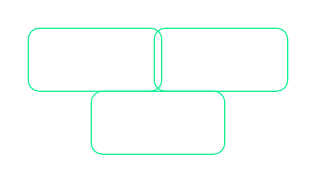
\begin{tikzpicture}[scale=0.8]
                % Partner logos placeholder (smaller, consistent size)
                \node[draw=solanagreen, rounded corners, minimum width=1.2cm, minimum height=0.8cm] at (0,0) {\textcolor{white}{Partner 1}};
                \node[draw=solanagreen, rounded corners, minimum width=1.2cm, minimum height=0.8cm] at (2,0) {\textcolor{white}{Partner 2}};
                \node[draw=solanagreen, rounded corners, minimum width=1.2cm, minimum height=0.8cm] at (1,-1) {\textcolor{white}{Partner 3}};
            \end{tikzpicture}
            
            \vspace{0.3cm}
            \begin{tabular}{rc}
                \textcolor{solanagreen}{\textbf{3}} & \textcolor{white}{DeFi protocols in discussions} \\
                \textcolor{solanagreen}{\textbf{2}} & \textcolor{white}{Market makers testing} \\
                \textcolor{solanagreen}{\textbf{Q3}} & \textcolor{white}{Testnet launch coming soon} \\
                \textcolor{solanagreen}{\textbf{500+}} & \textcolor{white}{Whitepaper downloads} \\
            \end{tabular}
        \end{center}
    \end{tcolorbox}
\end{columns}

\vspace{0.2cm}
\begin{center}
    \begin{tcolorbox}[colback=solanapurple!30, colframe=solanapurple, width=0.8\textwidth, arc=3mm]
        \centering
        \textcolor{white}{\textbf{"ShadowBook represents the next evolution in DeFi trading infrastructure"}}
    \end{tcolorbox}
\end{center}
\end{frame}

% Business Model
\begin{frame}[plain]
\begin{tikzpicture}[remember picture, overlay, scale=0.95]
    % Background with financial aesthetic
    \fill[left color=darkblue, right color=black] (current page.south west) rectangle (current page.north east);
    
    % Money symbols in background (reduced)
    \foreach \i in {1,...,12} {
        \pgfmathsetmacro{\x}{random(0,90)/10}
        \pgfmathsetmacro{\y}{random(0,60)/10}
        \pgfmathsetmacro{\op}{random(5,10)/100}
        \node[text=neonblue, opacity=\op] at (\x,\y) {\tiny{\$}};
    }
\end{tikzpicture}

\vspace{0.02cm}
\begin{center}
    \begin{tcolorbox}[colback=darkblue, colframe=neonblue, width=0.8\textwidth, arc=5mm, boxrule=1.5pt]
        {\fontsize{24}{26}\selectfont\textcolor{white}{\textbf{BUSINESS}} \textcolor{solanagreen}{\textbf{MODEL}}}
    \end{tcolorbox}
\end{center}

\vspace{0.02cm}
\begin{columns}[T,onlytextwidth]
    \column{0.48\textwidth}
    \begin{tcolorbox}[colback=darkblue!80, colframe=neonblue, width=\textwidth, arc=3mm, title=\textcolor{white}{\textbf{REVENUE STREAMS}}, boxsep=0.1cm]
        \begin{itemize}\setlength{\itemsep}{2pt}
            \item \textcolor{solanagreen}{\faPercent} \textcolor{white}{\textbf{Trading fees}}\\[-0.1cm]
            \textcolor{white}{\small 0.1-0.3\% per trade}\\[0.1cm]
            
            \item \textcolor{solanagreen}{\faRocket} \textcolor{white}{\textbf{Premium API}}\\[-0.1cm]
            \textcolor{white}{\small Tiered subscription model}\\[0.1cm]
            
            \item \textcolor{solanagreen}{\faBuilding} \textcolor{white}{\textbf{Enterprise integrations}}\\[-0.1cm]
            \textcolor{white}{\small Custom solutions for institutions}\\[0.1cm]
            
            \item \textcolor{solanagreen}{\faCoins} \textcolor{white}{\textbf{Liquidity mining}}\\[-0.1cm]
            \textcolor{white}{\small Incentivized participation}
        \end{itemize}
    \end{tcolorbox}
    
    \column{0.48\textwidth}
    \begin{tcolorbox}[colback=darkblue!80, colframe=neonblue, width=\textwidth, arc=3mm, title=\textcolor{white}{\textbf{KEY METRICS}}, boxsep=0.1cm]
        \begin{center}
            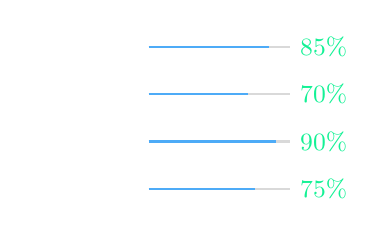
\begin{tikzpicture}[scale=0.6]
                % Simple gauge charts (simplified)
                \foreach \i/\label/\percent in {1/Volume/85, 2/Users/70, 3/Fill Rate/90, 4/Liquidity/75} {
                    \pgfmathsetmacro{\width}{\percent*0.03}
                    \draw[thick, gray!30] (0,-\i) -- (3,-\i);
                    \draw[thick, neonblue] (0,-\i) -- (\width,-\i);
                    \node[left] at (0,-\i) {\textcolor{white}{\small\label}};
                    \node[right] at (3,-\i) {\textcolor{solanagreen}{\small\percent\%}};
                }
            \end{tikzpicture}
        \end{center}
    \end{tcolorbox}
\end{columns}


\end{frame}

% Team
\begin{frame}[plain]
\begin{tikzpicture}[remember picture, overlay, scale=0.95]
    % Background with tech aesthetic
    \fill[left color=darkblue, right color=black] (current page.south west) rectangle (current page.north east);
    
    % Network pattern in background (reduced)
    \foreach \i in {1,...,8} {
        \pgfmathsetmacro{\x}{random(0,90)/10}
        \pgfmathsetmacro{\y}{random(0,60)/10}
        \pgfmathsetmacro{\xx}{\x+random(5,15)/10}
        \pgfmathsetmacro{\yy}{\y+random(5,15)/10}
        \draw[solanagreen, opacity=0.03, line width=0.5pt] (\x,\y) -- (\xx,\yy);
    }
\end{tikzpicture}

\vspace{0.2cm}
\begin{center}
    \begin{tcolorbox}[colback=darkblue, colframe=solanagreen, width=0.8\textwidth, arc=5mm, boxrule=1.5pt]
        {\fontsize{26}{28}\selectfont\textcolor{white}{\textbf{THE}} \textcolor{solanagreen}{\textbf{TEAM}}}
    \end{tcolorbox}
\end{center}

\begin{columns}[T,onlytextwidth]
    \column{0.48\textwidth}
    \begin{tcolorbox}[colback=darkblue!80, colframe=solanagreen, width=\textwidth, arc=3mm, boxsep=0.05cm]
        \begin{center}
            % Profile picture placeholder (smaller)
            
\begin{tikzpicture}[scale=0.4]
                \node[circle, draw=solanagreen, line width=1pt, minimum size=1.8cm] {\textcolor{white}{KK}};
            \end{tikzpicture}
            
            {\textcolor{solanagreen}{\textbf{Kyle Koshiyama}}}\\
            {\footnotesize\textcolor{neonblue}{Co-Founder \& CTO}}
        \end{center}
        
        \begin{itemize}\setlength{\itemsep}{0pt}
            \item[\textcolor{solanagreen}{\faCode}] \textcolor{white}{\textbf{Former Engineer at Fhenix}}
            \item[\textcolor{solanagreen}{\faLock}] \textcolor{white}{\textbf{FHE \& DeFi Expert}}
            \item[\textcolor{solanagreen}{\faBolt}] \textcolor{white}{\textbf{Solana Ecosystem Pioneer}}
            \item[\textcolor{solanagreen}{\faGraduationCap}] \textcolor{white}{\textbf{Cryptography Background}}
        \end{itemize}
    \end{tcolorbox}
    
    \column{0.48\textwidth}
    \begin{tcolorbox}[colback=darkblue!80, colframe=solanagreen, width=\textwidth, arc=3mm, boxsep=0.05cm]
        \begin{center}
            % Profile picture placeholder (smaller)
            
\begin{tikzpicture}[scale=0.4]
                \node[circle, draw=solanagreen, line width=1pt, minimum size=1.8cm] {\textcolor{white}{MC}};
            \end{tikzpicture}
            
            {\textcolor{solanagreen}{\textbf{Mads Christensen}}}\\
            {\footnotesize\textcolor{neonblue}{Co-Founder \& CEO}}
        \end{center}
        
        \begin{itemize}\setlength{\itemsep}{0pt}
            \item[\textcolor{solanagreen}{\faShieldAlt}] \textcolor{white}{\textbf{Former Engineer at Lit Protocol}}
            \item[\textcolor{solanagreen}{\faRobot}] \textcolor{white}{\textbf{Agent Security Expert}}
            \item[\textcolor{solanagreen}{\faUsers}] \textcolor{white}{\textbf{Secure MPC Specialist}}
            \item[\textcolor{solanagreen}{\faServer}] \textcolor{white}{\textbf{Distributed Systems Architect}}
        \end{itemize}
    \end{tcolorbox}
\end{columns}

\end{frame}

% Roadmap
\begin{frame}[plain]
\begin{tikzpicture}[remember picture, overlay, scale=0.95]
    % Background with tech aesthetic
    \fill[left color=darkblue, right color=black] (current page.south west) rectangle (current page.north east);
    
    % Road pattern in background (simplified)
    \draw[white, opacity=0.03, line width=4pt, dashed] (-1,4) -- (12,4);
\end{tikzpicture}

\vspace{0.2cm}
\begin{center}
    \begin{tcolorbox}[colback=darkblue, colframe=solanapurple, width=0.8\textwidth, arc=5mm, boxrule=1.5pt]
        {\fontsize{26}{28}\selectfont\textcolor{white}{\textbf{THE}} \textcolor{solanagreen}{\textbf{ROADMAP}}}
    \end{tcolorbox}
\end{center}

\vspace{0.3cm}
\begin{center}
\begin{tikzpicture}[scale=0.65,
    milestone/.style={draw=solanapurple, rounded corners=3mm, fill=darkblue!80, text width=1.8cm, align=center, minimum height=2.5cm},
    arrow/.style={->, >=stealth, thick, solanagreen, line width=1pt}
]
    % Timeline moved down
    \draw[solanapurple, line width=1.5pt] (0,-0.8) -- (13,-0.8);
    
    % Milestones moved slightly up
    \node[milestone] (q2) at (1.5,2.2) {
        \textcolor{solanapurple}{\textbf{Q2 2025}}\\[0.1cm]
        \textcolor{solanagreen}{\faRocket} \textcolor{white}{\textbf{Testnet}}\\[-0.1cm]
        \textcolor{white}{\footnotesize Launch}\\[0.1cm]
        \textcolor{solanagreen}{\faShieldAlt} \textcolor{white}{\textbf{Audits}}\\[-0.1cm]
        \textcolor{white}{\footnotesize Security}
    };
    
    \node[milestone] (q3) at (5,2.2) {
        \textcolor{solanapurple}{\textbf{Q3 2025}}\\[0.1cm]
        \textcolor{solanagreen}{\faBolt} \textcolor{white}{\textbf{Mainnet}}\\[-0.1cm]
        \textcolor{white}{\footnotesize Production}\\[0.1cm]
        \textcolor{solanagreen}{\faCoins} \textcolor{white}{\textbf{Liquidity}}\\[-0.1cm]
        \textcolor{white}{\footnotesize Mining}
    };
    
    \node[milestone] (q4) at (8.5,2.2) {
        \textcolor{solanapurple}{\textbf{Q4 2025}}\\[0.1cm]
        \textcolor{solanagreen}{\faLink} \textcolor{white}{\textbf{Cross-chain}}\\[-0.1cm]
        \textcolor{white}{\footnotesize Multi-chain}\\[0.1cm]
        \textcolor{solanagreen}{\faBuilding} \textcolor{white}{\textbf{Enterprise}}\\[-0.1cm]
        \textcolor{white}{\footnotesize API}
    };
    
    \node[milestone] (q1) at (12,2.2) {
        \textcolor{solanapurple}{\textbf{Q1 2026}}\\[0.1cm]
        \textcolor{solanagreen}{\faMobile} \textcolor{white}{\textbf{Mobile}}\\[-0.1cm]
        \textcolor{white}{\footnotesize App}\\[0.1cm]
        \textcolor{solanagreen}{\faCoins} \textcolor{white}{\textbf{Token}}\\[-0.1cm]
        \textcolor{white}{\footnotesize Governance}
    };
    
    % Timeline nodes moved down
    \foreach \x in {1.5, 5, 8.5, 12} {
        \node[circle, fill=solanapurple, minimum size=0.4cm] at (\x,-0.8) {};
    }
    
    % Connect milestones to timeline with longer lines
    \foreach \x in {1.5, 5, 8.5, 12} {
        \draw[solanapurple, line width=0.8pt] (\x,-0.8) -- (\x,0.4);
    }
\end{tikzpicture}
\end{center}

\vspace{0.1cm}
\begin{center}
    \begin{tcolorbox}[colback=darkblue!80, colframe=solanapurple, width=0.85\textwidth, arc=3mm, title=\textcolor{white}{\textbf{KEY MILESTONES}}, boxsep=0.05cm]
        \begin{columns}[T,onlytextwidth]
            \column{0.48\textwidth}
            \begin{itemize}\setlength{\itemsep}{0pt}
                \item[\textcolor{solanagreen}{\faTachometer}] \textcolor{white}{\textbf{10x FHE performance}}
                \item[\textcolor{solanagreen}{\faGasPump}] \textcolor{white}{\textbf{Lower settlement costs}}
            \end{itemize}
            
            \column{0.48\textwidth}
            \begin{itemize}\setlength{\itemsep}{0pt}
                \item[\textcolor{solanagreen}{\faBoxes}] \textcolor{white}{\textbf{Multi-asset support}}
                \item[\textcolor{solanagreen}{\faUserSecret}] \textcolor{white}{\textbf{Threshold encryption}}
            \end{itemize}
        \end{columns}
    \end{tcolorbox}
\end{center}
\end{frame}

% Conclusion
\begin{frame}[plain]
\begin{tikzpicture}[remember picture, overlay, scale=0.95]
    % Background with tech aesthetic
    \fill[left color=darkblue, right color=black] (current page.south west) rectangle (current page.north east);
    
    % Animated particles (reduced)
    \foreach \i in {1,...,20} {
        \pgfmathsetmacro{\x}{random(0,90)/10}
        \pgfmathsetmacro{\y}{random(0,60)/10}
        \pgfmathsetmacro{\r}{random(5,15)/100}
        \pgfmathsetmacro{\op}{random(10,20)/100}
        \node[circle, fill=solanagreen, opacity=\op, minimum size=\r cm] at (\x,\y) {};
    }
    
    % Lock icon in the background (scaled down)
    \node[opacity=0.15, scale=12, text=solanagreen] at (6,0) {\faLock};
\end{tikzpicture}

\vspace{0.2cm}
\begin{center}
    \begin{tcolorbox}[colback=darkblue, colframe=solanagreen, width=0.8\textwidth, arc=5mm, boxrule=1.5pt]
        {\fontsize{24}{26}\selectfont\textcolor{white}{\textbf{THE}} \textcolor{solanagreen}{\textbf{FUTURE}} \\[0.1cm] \textcolor{white}{\textbf{OF}} \textcolor{solanagreen}{\textbf{TRADING}}}
    \end{tcolorbox}
\end{center}

\vspace{0.3cm}
\begin{columns}[T,onlytextwidth]
    \column{0.48\textwidth}
    \begin{tcolorbox}[colback=darkblue!80, colframe=solanagreen, width=\textwidth, arc=3mm, title=\textcolor{white}{\textbf{WHY SHADOWBOOK WINS}}]
        \begin{itemize}
            \item \textcolor{solanagreen}{\faLock} \textcolor{white}{\textbf{Privacy-First Trading}}\\[-0.2cm]
            \textcolor{white}{\small Solving DeFi's biggest vulnerability}
            
            \item \textcolor{solanagreen}{\faBolt} \textcolor{white}{\textbf{Solana-Powered Speed}}\\[-0.2cm]
            \textcolor{white}{\small Fastest blockchain + FHE innovation}
            
            \item \textcolor{solanagreen}{\faUsers} \textcolor{white}{\textbf{Expert Team}}\\[-0.2cm]
            \textcolor{white}{\small Deep cryptography \& DeFi expertise}
            
            \item \textcolor{solanagreen}{\faChartLine} \textcolor{white}{\textbf{Massive Market}}\\[-0.2cm]
            \textcolor{white}{\small \$50B+ opportunity and growing}
        \end{itemize}
    \end{tcolorbox}
    
    \column{0.48\textwidth}
    \begin{center}
        \begin{tcolorbox}[colback=solanagreen!60, colframe=solanagreen, width=\textwidth, arc=5mm, boxrule=1pt, boxsep=0.05cm]
            {\fontsize{16}{18}\selectfont\textcolor{white}{\textbf{JOIN THE REVOLUTION}}}
            
            \vspace{0.05cm}
            \begin{center}
            \begin{tikzpicture}[scale=0.5]
                \node[circle, draw=white, line width=1pt, minimum size=2.5cm, opacity=1.0] at (0,0) {\textcolor{white}{\Large\faLock}};
            \end{tikzpicture}
            \end{center}
            
            \vspace{0.05cm}
            {\normalsize\textcolor{white}{\textbf{Try the demo today!}}}\\
            {\small\textcolor{white}{\url{fungerbil.com/fhe/landing/index.html}}}
        \end{tcolorbox}
    \end{center}
\end{columns}

\vspace{0.3cm}
\begin{center}
    \begin{tcolorbox}[colback=darkblue!80, colframe=solanagreen, width=0.8\textwidth, arc=3mm]
        \begin{center}
            \textcolor{solanagreen}{\large\faEnvelope} \qquad \textcolor{white}{\large info@shadowbook.xyz} \qquad \textcolor{solanagreen}{\large\faTwitter}
        \end{center}
    \end{tcolorbox}
    
    \vspace{0.2cm}
    \textcolor{white}{\textbf{SHADOWBOOK}} \textcolor{solanagreen}{|} \textcolor{white}{Solana Hackathon 2025}
\end{center}
\end{frame}

\end{document}
